\documentclass[lettersize,journal]{IEEEtran}

\usepackage{amsmath,amsfonts}
\usepackage{array}
\usepackage[caption=false,font=normalsize,labelfont=sf,textfont=sf]{subfig}
\usepackage{textcomp}
\usepackage{stfloats}
\usepackage{url}
\usepackage{graphicx}
\usepackage{cite}
\usepackage{xcolor}
\usepackage{balance}
\usepackage{booktabs}
\usepackage{tabularx}
\usepackage{ragged2e}
\usepackage{float}
\usepackage{algorithm}
\usepackage{algpseudocode}



\newcolumntype{Y}{>{\RaggedRight\arraybackslash}X}
\newcolumntype{P}[1]{>{\RaggedRight\arraybackslash}p{#1}}

\newcommand{\status}[1]{\textbf{#1}}

\begin{document}
	\title{Servo Characterization for the SOFIA Modular Kinetic
		Surface}
	
	\author{
		Marco Heimdal Castro Magaña, Alejandro Amador Franco, Karen Alejandra Guevara Vasquez, María Alicia Vela Contreras, Juan Pablo Contreras Quiñones,
		Jorge A. Lizarraga, Luis E. Gonzáles-Jiménez, Luis F. Luque-Vega
		
	\thanks{The authors are affiliated with the Instituto Tecnológico de Estudios Superiores de Occidente (ITESO), Tlaquepaque, Jalisco, Mexico.}
	}
	
	
	\markboth{Laboratory for the Development of Technological Solutions}
	{Servo Characterization for the SOFIA Modular Kinetic
		Surface}
	
	\maketitle
	
	
	\begin{abstract}
		The SOFIA modular kinetic surface consists of 16 electromechanical modules arranged in a honeycomb configuration, each actuated by two servomotors, requiring the coordinated control of 32 actuators. Differences in the dynamic response of these servomotors may affect the synchronization and positioning performance of the system. This work proposes an experimental methodology for characterizing the dynamic response of the two servomotors in a single SOFIA module, temporarily removed from the complete structure for testing. A removable crown-shaped measurement device incorporating limit switches is proposed to establish repeatable angular reference positions and record the time intervals associated with servo movement. The control architecture consists of an ESP32-C3 microcontroller and two PCA9685 PWM drivers, providing independent control of the 32 actuators in the complete system. The proposed methodology includes repeatedmovement tests under defined operating conditions, analysis of the measured response times, and evaluation of an appropriate dynamic model for
		estimating effective servomotor time constants. The experimental scope is limited to the two servomotors of the selected module, with the aim of establishing a measurement procedure for evaluating their dynamic behavior.
	\end{abstract}
	
	\begin{IEEEkeywords}
		Servomotor characterization, dynamic response, time constant estimation, limit switches, modular robotics, kinetic surfaces, ESP32-C3, PCA9685.
	\end{IEEEkeywords}
	
	
	\section{Introduction}
	
	\label{sec:intro}
	
	\IEEEPARstart{S}{OFIA} \linelabel{ln:intro1}is a modular robotic installation composed of 16
	mechatronic units arranged in a two-dimensional honeycomb configuration, with each
	unit providing two rotational degrees of freedom actuated by servomotors. The
	system aims to achieve coordinated control of the multiple actuators while
	enabling interaction through static and dynamic human gestures. For this
	purpose, SOFIA integrates embedded control, inter-module communication, and an
	external computer vision system for gesture recognition.
	
	\linelabel{ln:intro-cap}The SOFIA system requires the
	integration of mechanical actuation, servo control, embedded processing, and
	communication subsystems. \linelabel{ln:intro-32}Since each of the 16 units uses two servomotors, the
	complete demonstrator requires the coordinated control of 32 actuators and the
	generation of multiple PWM signals. The embedded controller must coordinate
	the desired actuator positions, while the communication architecture should
	support the future integration of additional SOFIA modules without
	significantly increasing wiring and control complexity. This work proposes an experimental method to estimate individual servo time constraints with a mechanical solution.
	
	\subsection{Problem Statement and Research Question}
	\linelabel{ln:problem-start}Standard low-cost micro-servos exhibit manufacturing tolerances that result in non-uniform actuation speeds and transient response times across different units. In a 16-unit, 32-actuator modular kinetic surface like SOFIA, driving all servos with uniform control signals creates dynamic motion desynchronization and mechanical stress during normal use.
	
	\linelabel{ln:research-question}To address this limitation, this work investigates the following research question: \textit{Can experimental estimation of individual servo mechanical time constants ($\tau_m$) and their integration into a trajectory controller improve dynamic positional synchronization across a 32-actuator kinetic surface?}
	
	\linelabel{ln:Objectives}This encompasses three primary objectives: (1) designing a PCB integrating an ESP32-C3 microcontroller, dual PCA9685 drivers, and RS-85 interfaces; (2) developing an automated micro-test protocol to capture step-response and extract individual time constants; and (3) integrating individual compensation parameters into the surface tracking controller to equalize dynamic settling times across all actuators.
	
	\begin{table*}[!t]
		\centering
		\caption{Comparative matrix of related shape-changing interface systems}
		\label{tab:related_work_matrix}
		\scriptsize
		
		\setlength{\tabcolsep}{3pt}
		\renewcommand{\arraystretch}{1.1}
		
		\begin{tabularx}{\textwidth}
			{@{}P{2.2cm} P{3cm} P{3cm} P{4cm} Y@{}}
			
			\toprule
			Reference & Method / technology & Metric / focus & Main result & Gap with respect to SOFIA \\
			\midrule
			
			Relief \cite{leithinger2010relief} &
			Array of 120 motorized pins, scalable low-cost control &
			Actuation density, hardware/software scalability &
			Continuous surface capable of rendering and animating 3D shapes, with per-pin input sensing &
			Translational actuation only (1 DOF per pin); no independent rotation per unit \\
			
			inFORM \cite{follmer2013inform} &
			Pin-based shape display on a pre-existing platform &
			Dynamic physical affordances and constraints, object manipulation &
			Real-time direct-touch interaction and physical rendering of content &
			Same translational limitation as Relief; centralized architecture, not modular per unit \\
			
			TRANSFORM \cite{ishii2015transform} &
			Three large-scale pin displays, kinetic energy as input &
			Aesthetic transformation from static furniture to dynamic system &
			Over one thousand pins coordinated in real-time wave motion &
			Installation-scale system; no per-module orientable control or distributed communication between units \\
			
			PneUI \cite{yao2013pneui} &
			Pneumatically actuated multi-layer soft composite materials &
			Integrated input sensing and shape output in the material itself &
			Four functional applications (phicons, mobile, case, lamp) with controllable shape change &
			Soft/pneumatic actuation, not discrete rotational motion; difficult to scale to precise angular control \\
			
			LineFORM \cite{nakagaki2015lineform} &
			Serial chain of one-DOF servo actuators &
			Line/curve-based interaction affordances &
			Cord, mobile, and body-constraint interfaces through line-shaped actuation &
			Serial (chain) configuration, not a two-dimensional array; 1 DOF per unit, not 2 \\
			
			ChainFORM \cite{nakagaki2016chainform} &
			Identical modules with servo, touch sensing, visual output and embedded processing &
			Hardware modularity and reconfigurability &
			Modular, reconfigurable platform with rich per-module I/O &
			Modularity demonstrated, but still a linear chain, not a 2D array with 2 DOF per node \\
			
			\bottomrule
			
		\end{tabularx}
	\end{table*}
	
	\subsection{Related shape-changing interface systems}
	\linelabel{ln:rw1}Motorized arrays have been widely explored as a mechanism for generating
	dynamic physical surfaces. Relief introduced an actuated tabletop composed of
	120 individually addressable motorized pins and emphasized a scalable hardware
	and software architecture \cite{leithinger2010relief}. This concept was
	extended through inFORM, where shape actuation was employed to generate dynamic
	physical affordances and constraints and to manipulate physical objects
	\cite{follmer2013inform}. At a larger scale, TRANSFORM explored the
	transformation of static physical structures into dynamic systems driven by
	streams of data and energy \cite{ishii2015transform}. These approaches
	demonstrate the potential of coordinated arrays of actuators, although their
	architectures primarily focus on large pin-based or installation-scale physical
	surfaces.
	
	\linelabel{ln:rw2}Alternative approaches have explored different actuation principles and
	modular configurations. PneUI demonstrated shape-changing interfaces based on
	pneumatically actuated soft composite materials, integrating sensing and active
	shape output within deformable structures \cite{yao2013pneui}. In contrast,
	LineFORM investigated electromechanical shape transformation through serial
	chains of one-degree-of-freedom servo actuators
	\cite{nakagaki2015lineform}. This concept evolved toward greater hardware
	modularity in ChainFORM, where identical modules incorporate motor actuation,
	sensing, visual output, and embedded processing
	\cite{nakagaki2016chainform}. These systems highlight modularity and
	distributed actuation as relevant design characteristics for reconfigurable
	physical interfaces.
	
	\linelabel{ln:rw-tab}The main technological characteristics and differences identified among the
	reviewed shape-changing interfaces are summarized in
	Table~\ref{tab:related_work_matrix}.
	
	\linelabel{ln:gap}In contrast to the reviewed shape-changing interfaces, SOFIA combines a
	two-dimensional honeycomb arrangement with two rotational degrees of freedom
	per unit. Unlike pin-based displays, which predominantly constrain motion to a
	single translational axis, or line-based modular systems organized as serial
	chains, each SOFIA unit can independently modify its orientation while
	remaining part of the same physical surface. This configuration introduces
	design challenges related to coordinated actuation, modularity, scalability,
	control architecture, electrical integration, and communication. Based on the
	reviewed literature, these characteristics were identified as relevant criteria
	for evaluating the technological architecture of the demonstrator.
	Table~\ref{tab:related_work_matrix} summarizes the comparative analysis of the
	reviewed systems, while Table~\ref{tab:benchmarking} contrasts SOFIA with the
	reviewed solutions using the established comparison criteria.
	
	\begin{table}[!t]
		\centering
		\caption{Benchmarking against related shape-changing systems}
		\label{tab:benchmarking}
		\scriptsize
		
		\setlength{\tabcolsep}{2pt}
		\renewcommand{\arraystretch}{1.05}
		
		\begin{tabularx}{\columnwidth}
			{@{}P{1.7cm} P{1.7cm} P{1.5cm} Y@{}}
			
			\toprule
			Solution & Configuration & DOF/ unit & Modularity / scalability\\
			\midrule
			
			inFORM \cite{follmer2013inform} &
			Pin array on fixed platform &
			1 (translational) &
			Low -- centralized control, not designed for modular expansion \\
			
			LineFORM / ChainFORM \cite{nakagaki2015lineform,nakagaki2016chainform} &
			Serial chain of modules &
			1 per module &
			Medium -- modular, but limited to a linear configuration \\
			
			PneUI \cite{yao2013pneui} &
			Pneumatic soft composite material &
			Continuous (non-discrete) &
			Low -- difficult to discretize into individually addressable nodes \\
			
			\textbf{SOFIA (proposed)} &
			2D array, honeycomb modules &
			\textbf{2 (rotational)} &
			\textbf{High -- I2C bus + RS-485 designed for future module expansion} \\
			
			\bottomrule
			
		\end{tabularx}
	\end{table}
	
	\linelabel{ln:opp}From the functional decomposition of the demonstrator and its comparison with
	the literature, several technological opportunities were identified. One is
	the development of a scalable control architecture capable of independently
	coordinating all actuators while reducing the processing load on the main
	controller. Another is the implementation of an inter-module communication
	architecture that allows multiple SOFIA modules to operate as part of a larger
	system. Additional opportunities include the implementation of
	software-defined motion limits and smoothing strategies to prevent abrupt
	servo movements and reduce mechanical stress.
	
	\linelabel{ln:focus}Based on these opportunities, this work focuses on defining and justifying a
	preliminary electronic and control architecture for the SOFIA demonstrator.
	The main areas considered are actuator control, PWM generation, embedded
	processing, inter-module communication, electrical compatibility, and
	scalability. These criteria provide the basis for the selection and
	experimental evaluation of the technologies used in the subsequent development
	stages of the SOFIA system.
	
	
	\section{Materials and Methods}
	\label{sec:methods}
	
	The SOFIA kinetic surface consists of 16 electromechanical modules arranged in a honeycomb configuration, each providing two rotational degrees of freedom actuated by MG90S servomotors \cite{sofia_architecture,mg90s}. Although the complete system incorporates 32 actuators, the experimental characterization proposed in this study is limited to the two servomotors of a single module removed from the SOFIA structure.
	
	The methodology is divided into three main stages: hardware configuration, experimental measurement, and dynamic response analysis. The first stage involves the selection and verification of the electronic components required for servomotor control, considering the established hardware requirements \cite{technical_session}. The second stage proposes the use of a removable crown-shaped measurement device equipped with limit switches to detect predefined angular positions during controlled movements. The third stage involves analyzing the recorded timing data and evaluating an appropriate dynamic model to estimate the effective time constant of each servomotor.
	
	The experimental procedure is intended to provide repeatable measurements under defined operating conditions. Relevant variables include the commanded angular displacement, movement direction, supply voltage, and measured time intervals.
	These variables will be considered when evaluating differences in the dynamic response of the two servomotors.
	
	The electronic architecture of the complete SOFIA system includes an ESP32-C3 microcontroller and two PCA9685 PWM drivers, which provide the 32 PWM channels required for actuator control \cite{sofia_architecture,esp32c3,pca9685}.
	However, only the two servomotors of the selected module will be evaluated experimentally in thisstudy.
	
	The main electrical, communication, and mechanical requirements of the SOFIA demonstrator are summarized in Table~\ref{tab:sofia_requirements}. These requirements are based on the system architecture and the established technical verification criteria \cite{sofia_architecture,technical_session}.
	
	\begin{table}[!t]
		\centering
		\caption{SOFIA Main Requirements}
		\label{tab:sofia_requirements}
		\scriptsize
		
		\setlength{\tabcolsep}{2pt}
		\renewcommand{\arraystretch}{1.05}
		
		\begin{tabularx}{\columnwidth}
			{@{}P{2.1cm} P{2.1cm} Y@{}}
			
			\toprule
			Requirement & Specification & Verification\\
			\midrule
			
			Power &
			5 V servo supply &
			Compatible with MG90S range \\
			
			Logic voltage &
			3.3 V MCU logic &
			Required for ESP32-C3 GPIO \\
			
			Communication &
			WiFi/Bluetooth + I2C &
			Supported by ESP32-C3 \\
			
			PWM control &
			32 servo channels, 50 Hz &
			Two PCA9685 drivers required \\
			
			Mechanical &
			16 modules, 2 DOF each &
			32 servos required \\
			
			\bottomrule
			
		\end{tabularx}
	\end{table}
	
	Figure~\ref{fig2} \linelabel{ln:sim_architecture} illustrates the system architecture and signal flow of the SOFIA demonstrator. Telemetry and motion commands are communicated wirelessly between a central host PC (equipped with an external vision camera) and the main PCB via Wi-Fi or Bluetooth protocols. Onboard processing is handled by an ESP32 microcontroller, which interfaces with two PCA9685 PWM drivers over $\text{I}^2\text{C}$ to control a total of 32 servos. Driver 1 manages channels CH1--CH16 (grey group), while Driver 2 addresses channels CH17--CH32 (blue group, labeled CH1--CH16 on the second module) across the Master Module actuator array. Interconnectivity between boards is planned using JST-VH connectors.
	
	
	\begin{figure}[!t]
		\centering
		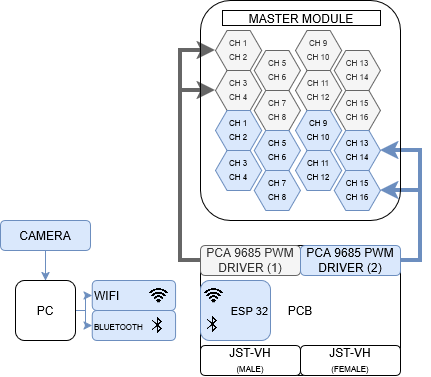
\includegraphics[width=2.4in]{figures/SOFIA_DIAGRAM}
		\caption{Block diagram describing SOFIA components and connections.}
		\label{fig1}
	\end{figure}
	
	\subsection{ESP32-C3 Technical Analysis}
	The main technical specifications of the ESP32-C3 microcontroller are presented in Table~\ref{tab:esp32_specs}.
	
	\begin{table}[!t]
		\centering
		\caption{ESP32-C3 Main Specifications and Datasheet Verification}
		\label{tab:esp32_specs}
		\scriptsize
		
		\setlength{\tabcolsep}{2pt}
		\renewcommand{\arraystretch}{1.1}
		
		\begin{tabularx}{\columnwidth}{@{}P{1.6cm} P{1.5cm} P{2.1cm} X X@{}}
			\toprule
			\textbf{Parameter} & \textbf{Value} & \textbf{Source (Doc / Ver / Pg)} & \textbf{Justification} & \textbf{Verification} \\
			\midrule
			
			Supply Voltage & 
			3.0--3.6 V & 
			ESP32-C3 Datasheet v2.4, p. 18 & 
			Match system main power operating limits & 
			Requires regulated 3.3 V supply \\
			
			Wi-Fi & 
			802.11 b/g/n & 
			ESP32-C3 Datasheet v2.4, p. 2 & 
			Enable 2.4 GHz wireless transmission & 
			Complies; integrated 2.4 GHz subsystem \\
			
			Bluetooth & 
			BLE 5 & 
			ESP32-C3 Datasheet v2.4, p. 2 & 
			Support low-energy configuration and monitoring & 
			Complies; Bluetooth LE 5.0 supported \\
			
			Logic Level & 
			3.3 V GPIO & 
			ESP32-C3 Datasheet v2.4, p. 19 & 
			Ensure digital signal levels meet peripheral logic thresholds & 
			5 V logic cannot be applied directly without level shifting \\
			
			Boot Pins & 
			GPIO2, 8, 9 & 
			ESP32-C3 Datasheet v2.4, p. 12 & 
			Prevent unintended strapping state selection during power-up & 
			PCB design hardware strapping verification required \\
			
			Temperature & 
			Up to 105 $^\circ$C & 
			ESP32-C3 Datasheet v2.4, p. 18 & 
			Ensure reliable continuous execution under thermal load & 
			Suitable for industrial and laboratory operating environments \\
			
			\bottomrule
		\end{tabularx}
	\end{table}
	
	\linelabel{ln:src-esp}Source: ESP32-C3 Datasheet, Espressif Systems. \cite{esp32c3}
	
	
	\subsection{PCA9685 Technical Analysis}
	The specifications of the PCA9685 PWM driver are summarized in Table~\ref{tab:pca9685_specs}.
	
	\begin{table}[!t]
		\centering
		\caption{PCA9685 Main Specifications and Datasheet Verification}
		\label{tab:pca9685_specs}
		\scriptsize
		
		\setlength{\tabcolsep}{2pt}
		\renewcommand{\arraystretch}{1.1}
		
		\begin{tabularx}{\columnwidth}{@{}P{1.5cm} P{1.4cm} P{2.2cm} X X@{}}
			\toprule
			\textbf{Parameter} & \textbf{Value} & \textbf{Source (Doc / Ver / Pg)} & \textbf{Justification} & \textbf{Verification} \\
			\midrule
			
			Channels & 
			16 PWM & 
			PCA9685 Datasheet Rev. 7.5, p. 1 & 
			Control multiple servos with minimal MCU pin overhead & 
			Two devices provide 32 outputs \\
			
			Resolution & 
			12 bits & 
			PCA9685 Datasheet Rev. 7.5, p. 1 & 
			High-precision duty-cycle control for smooth motion & 
			Complies; 4096-step resolution \\
			
			Interface & 
			$\text{I}^2\text{C}$ FM+ & 
			PCA9685 Datasheet Rev. 7.5, p. 1 & 
			Standardized serial bus compatible with host controller & 
			Compatible with ESP32-C3 $\text{I}^2\text{C}$ peripheral \\
			
			Supply Voltage & 
			2.3--5.5 V & 
			PCA9685 Datasheet Rev. 7.5, p. 52 & 
			Operate on standard 3.3 V logic power rail & 
			Uses 3.3 V logic power supply \\
			
			PWM Frequency & 
			24--1526 Hz & 
			PCA9685 Datasheet Rev. 7.5, p. 1 & 
			Match standard RC servo control signal requirements & 
			Configured to 50 Hz output frequency \\
			
			Addressing & 
			Up to 62 ICs & 
			PCA9685 Datasheet Rev. 7.5, p. 12 & 
			Support unique addressing for cascading multiple ICs & 
			Configured with distinct fixed addresses (0x40 and 0x41) \\
			
			\bottomrule
		\end{tabularx}
	\end{table}
	
	\linelabel{ln:src-pca}Source: PCA9685 Datasheet, NXP. \cite{pca9685}
	
	
	\subsection{MG90S Servo Technical Analysis}
	The nominal operating characteristics of the MG90S servomotor are presented in Table~\ref{tab:mg90s_specs}.
	
	\begin{table}[!t]
		\centering
		\caption{MG90S Main Specifications and Datasheet Verification}
		\label{tab:mg90s_specs}
		\scriptsize
		
		\setlength{\tabcolsep}{2pt}
		\renewcommand{\arraystretch}{1.1}
		
		\begin{tabularx}{\columnwidth}{@{}P{1.5cm} P{1.7cm} P{2.0cm} X X@{}}
			\toprule
			\textbf{Parameter} & \textbf{Value} & \textbf{Source (Doc / Ver / Pg)} & \textbf{Justification} & \textbf{Verification} \\
			\midrule
			
			Voltage & 
			4.8--6.0 V & 
			TowerPro MG90S documentation, p. 1 & 
			Match system 5 V main power & 
			Compatible with 5 V \\
			
			Torque & 
			1.8 kgf$\cdot$cm at 4.8 V; \newline 2.2 kgf$\cdot$cm at 6.0 V & 
			TowerPro MG90S documentation, p. 1 & 
			Provide required joint actuation torque under load & 
			1.88 kgf$\cdot$cm available at 5.0 V; validation required \\
			
			Speed & 
			0.10 s/60$^\circ$ at 4.8 V; \newline 0.08 s/60$^\circ$ at 6.0 V & 
			TowerPro MG90S documentation, p. 1 & 
			Ensure joint angular velocity meets dynamic motion profile & 
			Reference value; complies for target control loop speed \\
			
			Mass & 
			13.4 g & 
			TowerPro MG90S documentation, p. 1 & 
			Minimize total end-effector and leg inertia & 
			Must be considered in structural mass budget and CAD model \\
			
			PWM Frequency & 
			50 Hz & 
			TowerPro MG90S documentation, p. 1 & 
			Standard RC servo control signal frame timing (20 ms period) & 
			Compatible with PCA9685 PWM output driver \\
			
			Stall Current & 
			Not reported & 
			TowerPro MG90S documentation, p. 1 & 
			Sizing power supply current limits for worst-case loading & 
			Not specified in datasheet; physical current measurement required \\
			
			\bottomrule
		\end{tabularx}
	\end{table}
	
	\linelabel{ln:src-mg}Source: TowerPro MG90S documentation. \cite{mg90s}
	
	
	\subsection{Checklist Verification}
	The preliminary component compatibility assessment is summarized in Table~\ref{tab:verification}.
	
	\begin{table}[!t]
		\centering
		\caption{Verification Summary}
		\label{tab:verification}
		\scriptsize
		
		\setlength{\tabcolsep}{2pt}
		\renewcommand{\arraystretch}{1.05}
		
		\begin{tabularx}{\columnwidth}{@{}P{2cm} P{1.7cm} Y@{}}
			\toprule
			Component & Status & Comment\\
			\midrule
			
			ESP32-C3 & 
			\status{Complies} & 
			Requires 3.3 V regulation and boot verification \\
			
			PCA9685 & 
			\status{Complies} & 
			Requires unique I2C addresses and 50 Hz configuration \\
			
			MG90S & 
			\status{Partial} & 
			Torque and current require validation \\
			
			\bottomrule
		\end{tabularx}
	\end{table}
	
	\subsection{Bill of Materials}
	The components required for the SOFIA demonstrator,
	including mechanical parts, actuators, and electronic
	devices, are summarized in Table~\ref{tab:bom}.
	
	
	\begin{table}[!t]
		\centering
		\caption{SOFIA Demonstrator Bill of Materials (BOM) Summary}
		\label{tab:bom}
		\tiny
		
		\setlength{\tabcolsep}{1.5pt}
		\renewcommand{\arraystretch}{1.05}
		
		\begin{tabularx}{\columnwidth}{@{}P{0.8cm} P{2.0cm} c c X P{1.1cm} P{0.8cm}@{}}
			\toprule
			\textbf{Item} & \textbf{Component} & \textbf{Qty / Unit} & \textbf{Qty / Sys} & \textbf{Technical Description} & \textbf{Manufacturer} & \textbf{Location} \\
			\midrule
			
			1 & Sofia003-P001-03 & 1 & 16 & Sofia Module Base & In-house (LabDST) & ITESO, MX \\
			2 & MG90S / SG90 Servo & 2 & 32 & Micro Servo Motor & Tower Pro & Hong Kong \\
			3 & Sofia003-E002-01 & 1 & 16 & Lower Joint Subassembly & In-house (LabDST) & ITESO, MX \\
			3.1/4.4 & Pro3 & 2 & 32 & Servo Horn & Tower Pro & Hong Kong \\
			3.2 & Sofia003-P004-02 & 1 & 16 & Lower Joint Support Left & In-house (LabDST) & ITESO, MX \\
			3.3 & Sofia003-P004-03 & 1 & 16 & Lower Joint Support Right & In-house (LabDST) & ITESO, MX \\
			3.4/3.5/ 4.3/7/8 & M2 Screws (various) & 10 & 160 & Servo Arm Screw ($M2 \times 10/12$ mm) & Walfront & Shenzhen, CN \\
			3.6 & Axis 1 ($9 \times 9$ mm) & 1 & 16 & Joint Shaft ($9\text{ mm} \times 9\text{ mm}$) & Mae & Local \\
			3.7 & Sofia003-P002-02 & 1 & 16 & Lower Joint Link & In-house (LabDST) & ITESO, MX \\
			4 & Sofia003-E003-01 & 1 & 16 & Upper Joint Subassembly & In-house (LabDST) & ITESO, MX \\
			4.1 & Sofia003-P005-01 & 1 & 16 & Upper Joint Support Left & In-house (LabDST) & ITESO, MX \\
			4.2 & Sofia003-P005-02 & 1 & 16 & Upper Joint Support Right & In-house (LabDST) & ITESO, MX \\
			5 & Sofia003-P008-01 & 1 & 16 & Sofia Top Module Linkage & In-house (LabDST) & ITESO, MX \\
			6 & Sofia003-P009-01 & 1 & 16 & Top Platform Support & In-house (LabDST) & ITESO, MX \\
			9 & Inser M3x5x4 & 1 & 16 & M3 Threaded Insert ($5 \times 4$ mm) & ZWMSSLL & Shenzhen, CN \\
			10 & Sofia003-P000-01 & 1 & 16 & Sofia Hexagonal Top Platform & In-house (LabDST) & ITESO, MX \\
			\midrule
			-- & ESP32-C3 SuperMini & -- & 1 & Central MCU (Wi-Fi/BLE telemetry) & Espressif & Shanghai, CN \\
			-- & PCA9685 Servo Driver & -- & 2 & 16-channel 12-bit $\text{I}^2\text{C}$ PWM driver board & NXP Semi & Eindhoven, NL \\
			-- & MAX13487E TTL485 & 1 & 16 & Half-duplex RS-485 transceiver (1/module) & Analog Devices & Wilmington, US \\
			-- & LED RGB & -- & 1 & System state status indicator LED & Mexbit & Local \\
			-- & JST-VH Male & 1 & 1 & High-current power PCB header & JTAREA & Local \\
			-- & JST-VH Female & 1 & 1 & High-current power harness plug & JTAREA & Local \\
			
			\bottomrule
		\end{tabularx}
	\end{table}
	
	\subsection{Justification of Technological Selection}
	
	\begin{table}[!t]
		\centering
		\caption{Comparative Matrix of Alternatives}
		\label{tab:comparative_matrix}
		\scriptsize
		
		\setlength{\tabcolsep}{2pt}
		\renewcommand{\arraystretch}{1.05}
		
		\begin{tabularx}{\columnwidth}
			{@{}P{2cm} P{1.7cm} P{2cm} Y@{} }
			
			\toprule
			Function & Alternatives considered & Selected & Selection criterion \\
			\midrule
			
			Actuation & Servo / Stepper / DC & MG90S & Integrated angular positioning \\
			
			PWM generation & MCU PWM / PCA9685 / Additional MCU & PCA9685 & 16 PWM channels through I2C \\
			
			Processing & Arduino / STM32 / ESP32-C3 SuperMini & ESP32-C3 SuperMini & Wireless connectivity + required interfaces \\
			
			Inter-module communication & UART / CAN/ RS-485 & RS-485 & Differential multi-node communication \\
			
			
			\bottomrule
			
		\end{tabularx}
		
	\end{table}
	
	\linelabel{ln:sel}As summarized in Table~\ref{tab:comparative_matrix}, the technological
	architecture was selected according to the functional and scalability
	requirements of the SOFIA demonstrator. \linelabel{ln:sel-mg}MG90S servomotors were selected
	to provide controlled angular positioning for each degree of freedom,
	while two PCA9685 drivers provide the 32 PWM channels required by the
	system through a shared I2C bus. The ESP32-C3 SuperMini was selected as
	the main controller due to its integrated wireless connectivity and
	support for the required communication interfaces. \linelabel{ln:sel-rs485}Finally, RS-485 was
	selected for inter-module communication because its differential and
	multi-node architecture supports the future connection of multiple
	SOFIA modules.
	
	\subsection{Servo Mechanical Time Constant Estimation}
	The first-order dynamic model for the angular position response $\theta(t)$ to a step input is defined by:
	\begin{equation}
		\theta(t) = \theta_f + (\theta_0 - \theta_f) e^{-t / \tau_m}
		\label{eq:servo_first_order}
	\end{equation}
	where $\theta_0$ represents the initial angular position, $\theta_f$ denotes the commanded step target angle, and $\tau_m$ is the servo mechanical time constant. 
	
	To characterize $\tau_m$, no-load step responses of $60^\circ$ will be applied while measuring the transient velocity profile. As noted in Table~\ref{tab:mg90s_specs}, the manufacturer datasheet \cite{mg90s} lists nominal angular speed ($0.10\text{ s}/60^\circ$ at $4.8\text{ V}$ and $0.08\text{ s}/60^\circ$ at $6.0\text{ V}$) but omits the explicit value for $\tau_m$, necessitating experimental identification.
	
	\section{Design and Implementation of the Technological Solution}
	\label{sec:design}
	
	Figure~\ref{fig2} \linelabel{ln:sim}shows the simulated response of the sixteen-module SOFIA structure while tracking the moving point. The sequence illustrates each module reorientation at different instants, where each module adjusts its two rotational degrees of freedom to maintain alignment with  reference position.
	
	\begin{figure}[!t]
		\centering
		\subfloat[Step 1]{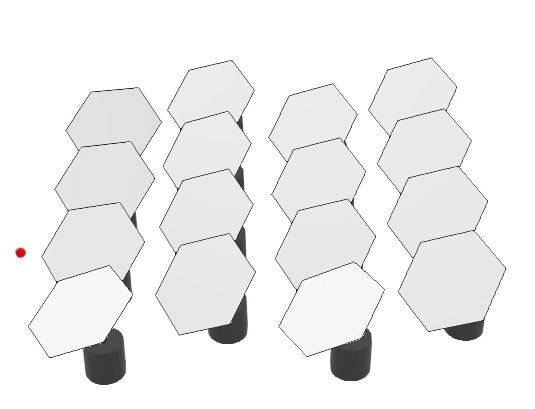
\includegraphics[width=1.1in]{figures/Sim_a}}
		\hfil
		\subfloat[Step 2]{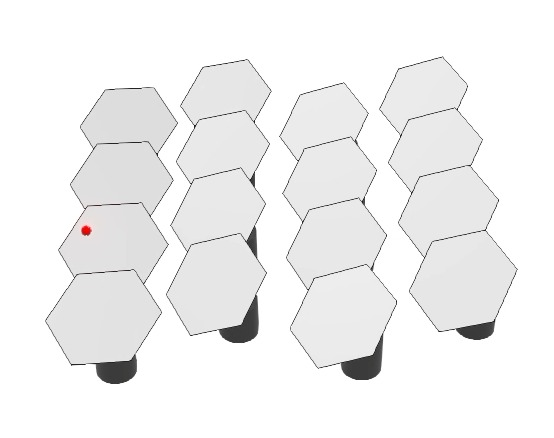
\includegraphics[width=1.1in]{figures/Sim_b}}
		\hfil
		\subfloat[Step 3]{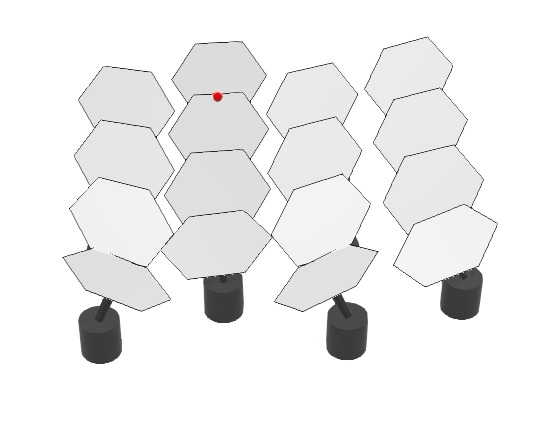
\includegraphics[width=1.1in]{figures/Sim_c}}
		\hfil
		\subfloat[Step 4]{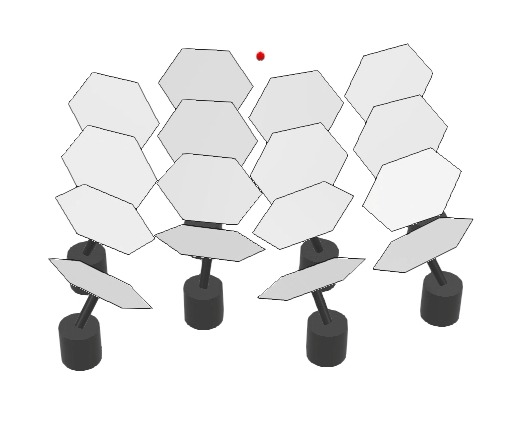
\includegraphics[width=1.1in]{figures/Sim_d}}
		\hfil
		\subfloat[Step 5]{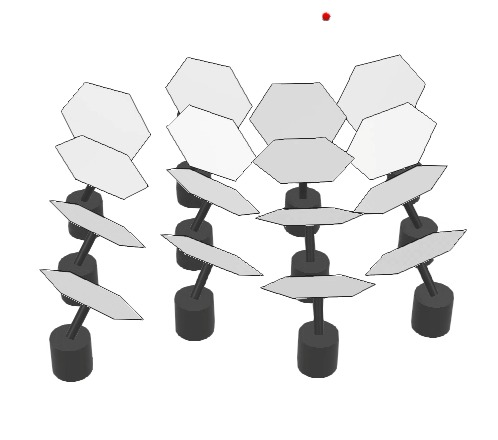
\includegraphics[width=1.1in]{figures/Sim_e}}
		\hfil
		\subfloat[Step 6]{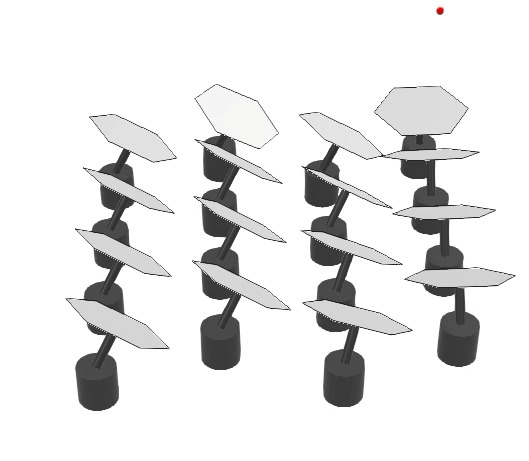
\includegraphics[width=1.1in]{figures/Sim_f}}
		\caption{Simulation of the SOFIA module tracking a moving reference point using inverse kinematics.}
		\label{fig2}
	\end{figure}
	
	Algorithm~\ref{alg:sofia_tracking} \linelabel{ln:alg}summarizes the inverse kinematics and smoothing strategy used by each SOFIA module to orient its platform toward the moving target.
	
	\begin{algorithm}[!t]
		\caption{SOFIA module target tracking control}
		\label{alg:sofia_tracking}
		
		
		\begin{algorithmic}[1]
			
			\Require Target position $\mathbf{p}$, module base position $\mathbf{r}_{0,2}$, joint limits $[q_{1\min}, q_{1\max}]$ and $[q_{2\min}, q_{2\max}]$, EMA smoothing factor $\alpha \in (0, 1]$
			\Ensure Servo command angles $q_1, q_2$
			
			\State $\mathbf{v} \gets \mathbf{p} - \mathbf{r}_{0,2}$
			\State $\hat{\mathbf{r}}_{2,p} \gets \frac{\mathbf{v}}{\|\mathbf{v}\|} = [u_x, u_y, u_z]^\top$ 
			
			\State $q_1^* \gets \operatorname{atan2}(-u_y, u_z)$
			\State $q_2^* \gets \arcsin(u_x)$ 
			
			\State $q_1^* \gets \Call{ClampAngle}{q_1^*, q_{1\min}, q_{1\max}}$
			\State $q_2^* \gets \Call{ClampAngle}{q_2^*, q_{2\min}, q_{2\max}}$
			
			\State $q_1 \gets q_{1,\text{old}} + \alpha (q_1^* - q_{1,\text{old}})$ \Comment{First-order EMA low-pass filter update}
			\State $q_2 \gets q_{2,\text{old}} + \alpha (q_2^* - q_{2,\text{old}})$
			
			\State Apply $q_1, q_2$ to servo motors
			
			\State \Return $q_1, q_2$
			
		\end{algorithmic}
	\end{algorithm}
	
	
	\section{Results}
	\label{sec:results}
	
	\subsection{Experimental Setup}
	
	\subsection{Servomotor Dynamic Response}
	
	\subsection{Time Constant Estimation}


	\section{Discussion}
	\label{sec:discussion}
	
	\section{Conclusions}
	\label{sec:conclusions}
	
	
	
	\balance
	
	\bibliographystyle{IEEEtran}
	\bibliography{bibliography}
	
\end{document}